\chapter{Introduzione} \label{introduzione}
In questo primo capitolo si introduce la differenza tra guida autonoma e guida remota, le tecnologie IOT e si descrive lo scopo del presente elaborato

\section{Guida remota e guida autonoma}
La guida autonoma e la guida remota sono due tecnologie che promettono di trasformare radicalmente il modo in cui ci muoviamo, rendendo i trasporti più sicuri, efficienti e sostenibili, e stanno al centro di una rivoluzione tecnologica: la mobilità intelligente.

\noindent La guida autonoma rappresenta un complesso sistema tecnologico che integra una serie di avanzate tecnologie, metodologie e tecniche finalizzate a consentire il movimento di un veicolo senza necessità di intervento umano diretto. Un veicolo autonomo è infatti dotato della capacità di analizzare l'ambiente circostante, elaborare un percorso ottimale in base ai dati raccolti, e seguire tale percorso in modo autonomo. 

\noindent Secondo la Society of Automotive Engineers international (SAE)\cite{SAE_autonomous_vehicle} il concetto di guida autonoma si può dividere in 6 livelli:

\begin{itemize}
  \item Livello 0: Il veicolo non ha capacità di guida autonoma e tutta la responsabilità è conferita al guidatore  
  \item Livello 1: Il veicolo assiste il guidatore in maniera limitata, agendo su acceleratore, freno e sterzo. La responsabilità rimane però completamente nelle mani dell'umano 
  \item Livello 2: Il veicolo ha le capacità di controllare simultaneamente la direzione, l'accelerazione e la frenata, ma il guidatore deve sempre e comunque rimanere vigile e monitorare le scelte prese dal veicolo
  \item Livello 3: Il veicolo può prendere completamente il controllo della guida ma solo in determinate situazioni (e.g. in autostrada) e il conducente deve essere pronto a prendere il controllo quando richiesto dal sistema
  \item Livello 4: Il veicolo può gestire tutte le funzioni di guida in maniera autonoma in quasi tutte le condizioni, ma può comunque richiedere l'intervento umano in situazioni straordinarie (e.g. zone non mappate)
  \item Livello 5: Il veicolo è completamente autonomo e non necessita di intervento umano
\end{itemize}

\noindent I processi fondamentali della guida autonoma vengono generalmente suddivisi in tre fasi distinte: percezione (perception), pianificazione (planning) e controllo (control).
La percezione riguarda la capacità del veicolo di raccogliere informazioni dall'ambiente circostante attraverso sensori avanzati, che possono includere telecamere, radar, Lidar e altre tecnologie di rilevamento. Questi dati vengono poi elaborati nella fase di pianificazione, durante la quale il sistema valuta le possibili traiettorie e sceglie il percorso più sicuro ed efficiente da seguire. Infine, la fase di controllo si occupa dell'esecuzione del movimento del veicolo lungo il percorso stabilito, garantendo che vengano seguite le decisioni prese nella fase di pianificazione.

\begin{figure}[H]
  \centering
  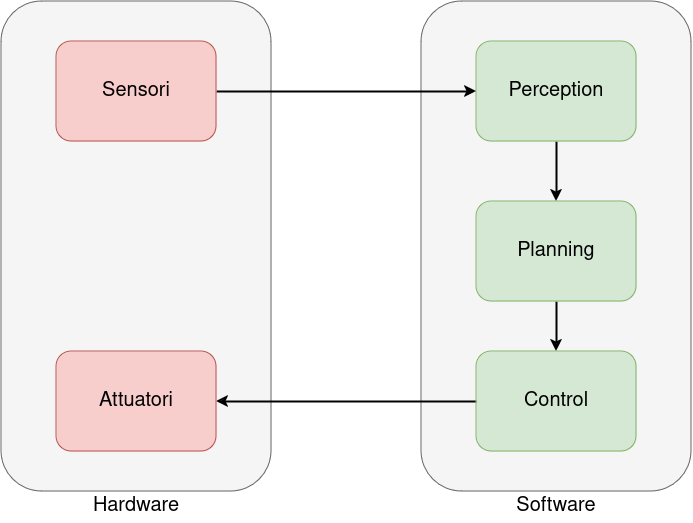
\includegraphics[width=0.6\textwidth]{figures/guida_autonoma.png}
  \caption{Semplice stack di guida autonoma}
  \label{guida_autonoma}
\end{figure}

\noindent Se nella guida autonoma le decisioni vengono elaborate da un sistema informatico a bordo del veicolo, il concetto di guida remota si riferisce a un tipo di guida in cui le decisioni relative alla direzione e al movimento del veicolo vengono elaborate in remoto. A seconda della strategia con la quale vengono prese queste decisioni, la guida remota si suddivide in:

\begin{itemize}
    \item Driver: le decisioni relative alla direzione e al movimento del veicolo vengono prese da un operatore umano che opera a distanza, capace di osservare i dati rilevati dai sensori presenti a bordo del mezzo
    \item Driverless: le decisioni vengono prese da uno stack di guida autonoma eseguito da un server remoto che prende in input i dati rilevati dai sensori presenti a bordo del mezzo e trasmette al veicolo istruzioni puntuali sul movimento da compiere 
\end{itemize}

\begin{figure}[H]
  \centering
  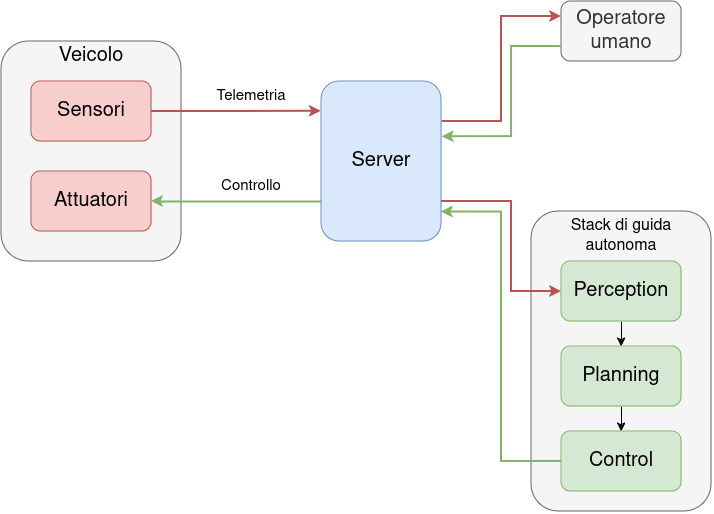
\includegraphics[width=0.7\textwidth]{figures/guida_remota.png}
  \caption{Semplice stack di guida remota}
  \label{guida_remota}
\end{figure}

\noindent La guida remota opera utilizzando tecnologie quali sensori, attuatori, e reti di comunicazione. In questo scenario, la logica che impartisce ordini non si trova fisicamente all'interno del veicolo, ma interagisce con esso attraverso un'interfaccia remota, sfruttando la trasmissione dei dati in tempo reale per monitorarlo e controllarlo. Tale approccio rende possibile la guida di veicoli in situazioni in cui la presenza fisica del conducente potrebbe non essere necessaria o praticabile

\section{Tecnologie IOT}
L'avvento dell'Internet of Things (IoT) ha inaugurato una nuova era tecnologica, caratterizzata dalla connettività pervasiva e dall'intelligenza distribuita. Questa rivoluzione digitale sta trasformando profondamente numerosi settori, tra cui la logistica. La crescente complessità delle catene di approvvigionamento globali, unita alla crescente domanda di efficienza e tracciabilità, rende l'IoT una tecnologia sempre più strategica per le aziende del settore.

\noindent L'IoT è un concetto che descrive una rete di dispositivi fisici connessi tra loro attraverso Internet, che sono capaci di scambiare dati e di comunicare con altri dispositivi, sistemi e/o servizi. Questi dispositivi, che possono includere sensori, elettrodomestici, veicoli (come nel nostro caso), sistemi di sicurezza, macchinari industriali e molto altro, sono dotati di sensori, software e altre tecnologie che permettono loro di raccogliere e condividere dati in tempo reale.

\noindent La guida remota, ovvero la possibilità di controllare un veicolo a distanza attraverso una connessione di rete, rappresenta una delle applicazioni più promettenti dell'IoT nel settore dei trasporti.

\section{Scopo della tesi}
L'obiettivo principale di questa tesi è quello di sviluppare un sistema di guida capace di operare sia in modo autonomo che in modalità di guida remota.

\noindent Si consideri lo scenario in cui il veicolo e l'hardware a bordo siano intatti e che il conducente sia sempre vigile, controllando il comportamento del mezzo anche in caso di errore o malfunzionamento. Su richiesta del conducente, il sistema potrà operare in questo caso in modalità autonoma.

\noindent Supponiamo ora che il guidatore non sia nelle sue condizioni ottimali e che, per esempio, a causa di un malore, non possa rimanere vigile e controllare adeguamente il veicolo. In questo caso, un ente terzo sarà in grado collegarsi al veicolo, passare alla modalità remota e mettere in sicurezza l'operatore conducendolo eventualemte all'ospedale più vicino.

\noindent Questo approccio duale consente al veicolo di navigare in modo completamente indipendente quando le circostanze lo permettono, utilizzando tecnologie di percezione, pianificazione e controllo integrate, ma offre al contempo la flessibilità di essere controllato a distanza da un operatore umano o da uno stack di guida autonoma qualora la situazione lo richieda. La possibilità di commutare tra guida autonoma e remota mira a garantire la massima sicurezza, adattabilità e versatilità del veicolo in una varietà di scenari operativi.

